%%%%%%%%%%%%%%%%%%%%%%%%%%%%%%%%%%%%%%%%%%%%%%%%%%%%%%%%%%%%%%%%%%%%%%%%
% Plantilla LaTeX para el trabajo en equipo a desarrollar en Modularidad
% Versión 1.0 (2022/03/31)
%
% Autor:
% Esther L. Silva Ramírez (esther.silva@uca.es)
% 
% Licencia:
% CC BY-NC-SA 4.0 (http://creativecommons.org/licenses/by/4.0/)
%%%%%%%%%%%%%%%%%%%%%%%%%%%%%%%%%%%%%%%%%%%%%%%%%%%%%%%%%%%%%%%%%%%%%%%%


% ----------------------------------------------------------------------
% PAQUETES Y CONFIGURACIÓN DE PÁGINA
% ----------------------------------------------------------------------

\documentclass[a4paper, 12pt]{report} %Tamaño de página A4 y tamaño de fuente 12pt

%\usepackage[utf8]{inputenc}
%\usepackage[cp1252]{fontenc}
\usepackage[spanish,activeacute]{babel}

\includeonly{Portada, Introduc, DocUsuario, DocSistema, DocCode, Referencias}

\usepackage{natbib}
\setcounter{secnumdepth}{3} %Para enumerar subsecciones de subsecciones (3.2.3).
\usepackage{xcolor, graphicx} %Insertar figuras
\usepackage{xcolor}
\usepackage{listingsutf8} %Insertar código fuente
\usepackage[breaklinks=true]{hyperref} %Para insertar hiperenlaces en palabras.
\usepackage{tocbibind}
\usepackage{pdfpages} %Para incluir pdfs.

\renewcommand{\thesection}{\arabic{section}} %Renumerar las secciones

\begin{document}

\renewcommand{\bibname}{Referencias}


%-----------------------------------------------------------------------
% PORTADA 
% -----------------------------------------------------------------------

% Se incluye la portada contenida en un fichero .tex
%%%%%%%%%%%%%%%%%%%% PORTADA %%%%%%%%%%%%%%%%%%%%

\begin{titlepage}
  
  \begin{minipage}{14cm}
    \center

    
\includegraphics[width=4cm,height=2cm]{FOTOS/uca}
    \hspace{2cm}
    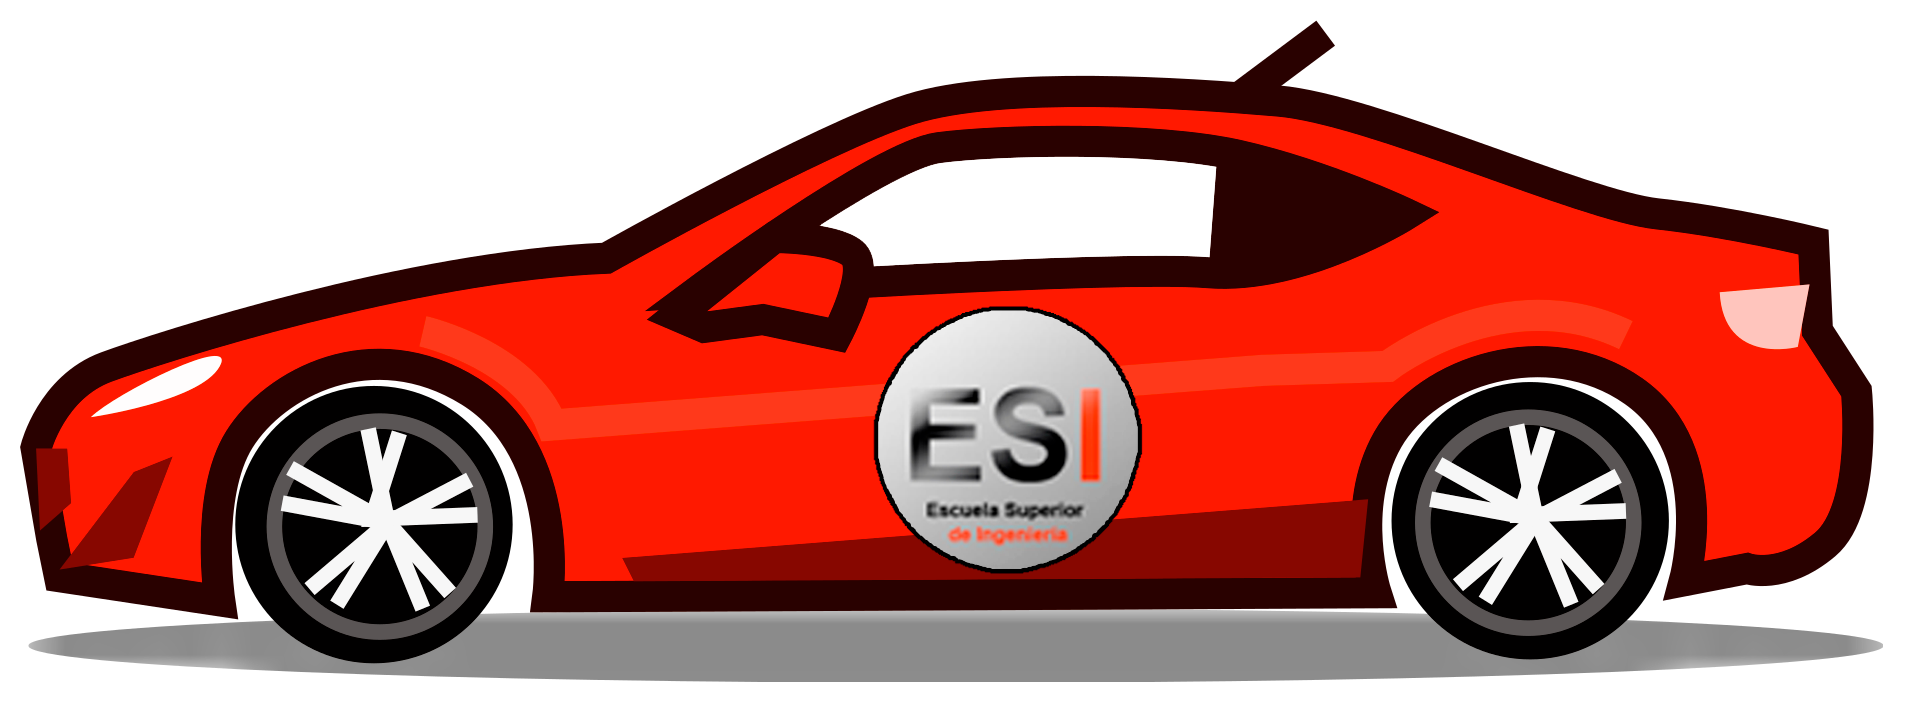
\includegraphics[width=5cm,height=2cm]{FOTOS/logo_ESI-SHARE.png}\\[1cm]
  
    {\Huge\bfseries Metodología de la Programación}\\[1\baselineskip]
    {\huge\textit{Grado en Ingeniería Informática}}\\[1\baselineskip]
    {\large Curso 2022/2023}\\[2\baselineskip]
    
    {\large {Durán Obregón, Alejandro}}\\[0.3cm]
    {\large {Ruíz Miñán, José Antonio}}\\[0.3cm]
    {\large {Ruíz del Pino, Alejandro}}\\[0.3cm]
    {\large {Vázquez Vera, Luis Enrique}}\\[0.3cm]

    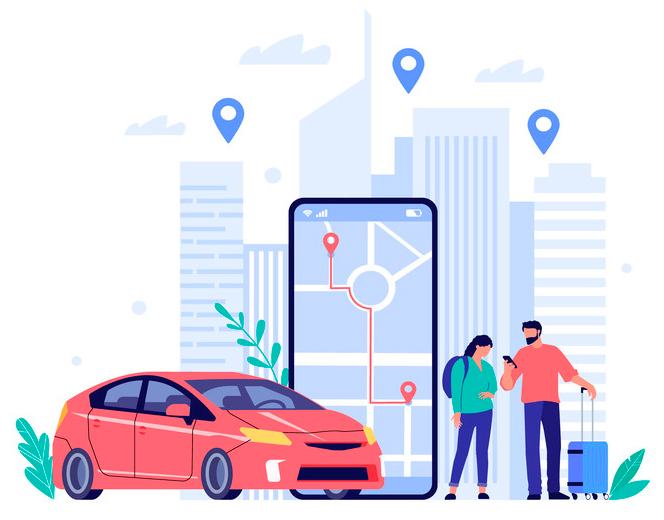
\includegraphics[width=7.7cm,height=6cm]{FOTOS/logo}\\[1cm]
    
    {\Large\textit{Proyecto Modularidad}}\\[1\baselineskip]
    {\Large\textbf{ESI-SHARE}}\\
    
  \end{minipage}
 
\end{titlepage}

\thispagestyle{empty}


%-----------------------------------------------------------------------
% ÍNDICE DE CONTENIDOS
%-----------------------------------------------------------------------

\setcounter{tocdepth}{3} %Para incluir subsecciones de subsecciones
\tableofcontents   %Incorpora el índice

%\listoftables  %Incorpora el índice para tablas, si las hubiere   

%\listoffigures  %Incorpora el índice para figuras, si las hubiere


\newpage

% A partir de aquí el resto del documento, el cuál ha sido dividido en distintos ficheros para facilitar la organización y la compilación del mismo.


%-----------------------------------------------------------------------
% INTRODUCCIÓN
% -----------------------------------------------------------------------

%%%%%%%%%%%%%%%%%%%% Introducción %%%%%%%%%%%%%%%%%%%%


\section{Introducción}

\begin{center}
\textbf{¿Eres parte de la comunidad universitaria de la Escuela Superior de Ingeniería y buscas una alternativa de transporte sostenible y económica?}\\
\end{center}
\begin{center}
\textbf{¿Te gustaría compartir tu vehículo con otros miembros de la comunidad que recorran la misma ruta?}\\
\end{center}
Si es así, estás de suerte, ya que hemos desarrollado un programa para compartir coche, que es exclusivo para los miembros de la comunidad de la ESI.

\bigskip

¿Cómo funciona? Es fácil, ESI-SHARE cuenta con una interfaz amigable e intuitiva que facilita la gestión de los viajes compartidos.  Los usuarios pueden registrar sus
viajes y especificar la ruta y horario, así como el número de plazas disponibles en su vehículo, para otros miembros de la comunidad que compartan la misma ruta.
También, pueden buscar viajes disponibles que se ajusten a sus necesidades y reservarlos. Todo esto con el objetivo de reducir el número de vehículos en circulación,
y disminuir el impacto ambiental del transporte.

\bigskip

En definitiva, esta es una herramienta innovadora que contribuye al fomento de la movilidad sostenible y al cuidado del medio ambiente, a la vez que
promueve la colaboración y el uso eficiente de los recursos.
\bigskip
\begin{center}
\textbf{¿Te animas a probarlo?}
\end{center}

%-----------------------------------------------------------------------
% CUERPO DEL DOCUMENTO
%-----------------------------------------------------------------------

%%%%%%%%%%%%%%%%%%%% Documentación del usuario %%%%%%%%%%%%%%%%%%%%

\section{Documentación de usuario}

\subsection{Descripción funcional}

Este programa ha sido creado con la finalidad de brindar un servicio de compartición de coches a los miembros de la comunidad universitaria de la Escuela Superior de Ingeniería. 
Con esto, se conseguirá una gran reducción de los costes diarios de transportes, al igual que una significante disminución de gases.

\bigskip

Como hemos comentado anteriormente, queremos dar un servicio de calidad, es por esto que con nuestro programa usted podrá realizar diferentes acciones, como:
\begin{itemize}
  \item Siendo \textbf{Pasajero} se le permitirá:
  \begin{itemize}
    \item Consultar y variar sus datos personales.
    \begin{center}
    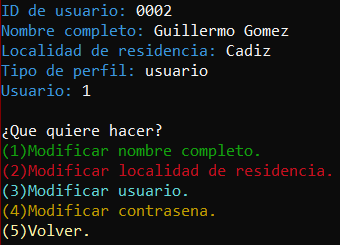
\includegraphics[]{FOTOS/menuPasajeroPerfil.png}
    \end{center}
    \item Reservar y cancelar viajes.
    \begin{center}
    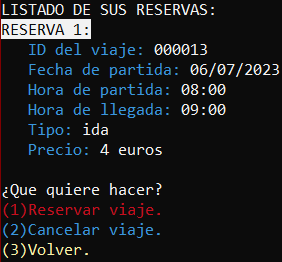
\includegraphics[]{FOTOS/menuPasajeroViaje.png}
    \end{center}
  \end{itemize}
  \item Siendo \textbf{Conductor} se le permitirá:
  \begin{itemize}
    \item Consultar y cambiar sus datos personales.
    \begin{center}
    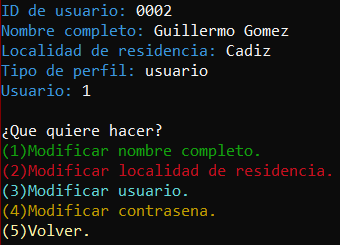
\includegraphics[]{FOTOS/menuPasajeroPerfil.png}
    \end{center}
    \item Dar de alta, modificar y eliminar vehículos.
    \begin{center}
    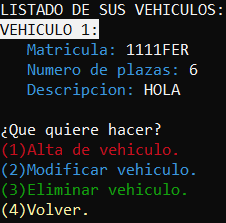
\includegraphics[]{FOTOS/menuConductorVehiculo.png}
    \end{center}
    \item Crear, modificar, anular y finalizar viajes.
    \begin{center}
    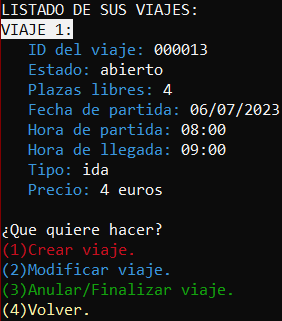
\includegraphics[]{FOTOS/menuConductorViaje.png}
    \end{center}
  \end{itemize}
  \item Siendo \textbf{Administrador} se le permitirá:
  \begin{itemize}
    \item Crear, descartar, cambiar y listar usuarios.
    \begin{center}
    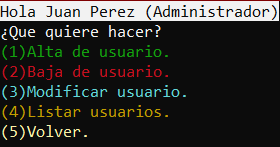
\includegraphics[]{FOTOS/menuAdminUsuario.png}
    \end{center}
    \item Dar de alta, suprimir, variar y listar vehículos.
    \item Establecer, anular, finalizar, cancelar, modificar y listar viajes.
  \end{itemize}
\end{itemize}

\bigskip

\subsection{Tecnología}

Este programa lo hemos realizado con el entorno de desarrollo integrado (IDE) \href{https://www.codeblocks.org/}{Code::Blocks}, en su versión 20.03.
A la hora de programar, hemos tenido que emplear diferentes bibliotecas, como:
\begin{itemize}
  \item stdio.h: Manejar la entrada y salida de datos a través de archivos, dispositivos de entrada/salida estándar, etc.
  \item string.h: Usar cadenas de caracteres.
  \item stdlib.h: Emplear estructuras, memoria dinámica, conversión de cadenas, etc.
  \item wchar.h: Manipular cadenas de caracteres Unicode.
  \item locale.h: Proporcionar el uso de caracteres especiales de un idioma.
  \item windows.h: Incluir comandos del sistema operativo Microsoft Windows.
  \item conio.h: Utilizar la entrada y salida de caracteres por la consola.
  \item time.h: Trabajar con fechas y tiempos.
\end{itemize}

\bigskip

Por ejemplo, se han empleado vectores con estructuras dinámicas, o incluso matrices/vector de vectores dinámicos. Esto se puede observar en el módulo reservar.
También se ha hecho uso de ficheros temporales, para eliminar/modificar, como se puede ver en en los módulos eliminar y modificar.

\subsection{Manual de instalación}

Para usar el programa, sólo tiene que dirigirse a la carpeta ESI-SHARE. Ahí encontrará un archivo ejecutable, llamado ESI-SHARE.exe, con el que podrá ejecutar el programa.
Otra forma sería instalar \href{https://www.codeblocks.org/}{Code::Blocks}, y ejecutar el archivo de proyecto ESI-SHARE.cbp.

\subsection{Acceso al sistema}

Tras haber iniciado el programa, se encontrará un menú, en el que encontrará dos opciones, una para acceder al sistema, si ya tiene unas credenciales, y otra para registrarse,
que le pedirá sus datos personales, para darse de alta. Si quiere testear el acceso al sistema, puede introducir:
\begin{itemize}
  \item Para acceder como usuario:
  \begin{itemize}
    \item Usuario: \textbf{usua1}
    \item Contraseña: \textbf{2023}
  \end{itemize}
  \item Para acceder como administrador:
  \begin{itemize}
    \item Usuario: \textbf{admin}
    \item Contraseña: \textbf{1234}
  \end{itemize}
\end{itemize}

A la hora de salir, se ha elaborado un mecanismo intuitivo y sencillo, ya que en todo momento podrá volver al menú anterior, introduciendo el número indicado por pantalla.
En el caso de querer salir totalmente del programa, tendrá que cerrar sesión, volviendo al menú principal.
\begin{center}
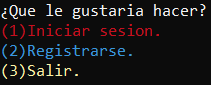
\includegraphics[]{FOTOS/menuPrincipal.png}
\label{fig:menuPrincipal}
\end{center}

\subsection{Manual de referencia}

El programa le puede aportar un gran ahorro de dinero en desplazamientos, debido al óptimo sistema de reservas que desempeña, haciendo posible que cualquier estudiante, profesor o personal
de la Escuela Superior de Ingeniería, pueda acceder a dichas ventajas.

\bigskip

Cuando ejecute al programa, podrá acceder con sus credenciales, o registrarse. Si accede con sus credenciales, tendrá las opciones de ser "Pasajero" ó "Conductor", 
dependiendo de lo que quiera hacer, seleccionará uno u otro, esto se puede cambiar en cualquier momento, volviendo a dicho menú. \ref{fig:menuPrincipal}

\begin{itemize}
  \item Si elige la opción de ser \textbf{Pasajero}, podrá:
  \begin{itemize}
    \item Entrar en el menú de \textbf{Perfil}, donde puede ver todos sus datos personales, al igual que si selecciona una de las opciones, podrá modificar cada uno de sus datos.
    \item Acceder al menú de \textbf{Viajes}, en el que se le permitirá reservar un viaje ya existente que pase por su localidad, al igual que cancelar cualquier reserva.
  \end{itemize}
  \item Si elige la opción de ser \textbf{Conductor}, podrá:
  \begin{itemize}
    \item Entrar en el menú de \textbf{Perfil}, donde puede ver todos sus datos personales, al igual que si selecciona una de las opciones, podrá modificar cada uno de sus datos.
    \item Pasar al menú de \textbf{Vehículos}, para introducir nuevos vehículos, modificarlos o incluso eliminarlos. Para esto, la matrícula del vehículo no puede existir en la base de datos.
    \item Acceder al menú de \textbf{Viajes}, en el que se le permitirá crear un viaje nuevo, siempre y cuando no haya dos abiertos en el mismo día, habría que acabar uno para empezar el siguiente,
    todo esto con el objetivo de que no se solapen los viajes. Además, se pueden modificar los viajes, si estos están abiertos y sin plazas reservadas, e incluso anular ó finalizar los viajes,
    esta selección la hará automáticamente el sistema, dependiendo del estado del viaje.
  \end{itemize}
\end{itemize}

Asimismo, hay un menú especial, si accede con las credenciales del \textbf{Administrador}. En este menú, tendrá acceso a todo tipo de información de la base de datos, como:
\begin{itemize}
  \item Entrar en el menú de \textbf{Usuarios}, donde puede crear un usuario desde cero, eliminar cualquier usuario del sistema, modificar los datos personales de cualquiera,
  e incluso obtener una lista con todos los usuarios que hay en el sistema.
  \item Pasar al menú de \textbf{Vehículos}, para dar de alta nuevos vehículos, eliminar un vehículo, modificar los datos de un vehículo, imprimir una lista de todos los vehículos que hay registrados
  al igual que obtener el historial de todos los viajes que ha realizado un vehículo, a partir de su matrícula.
  \item Acceder al menú de \textbf{Viajes}, en el que se le permitirá registrar un viaje, anular/finalizar, eliminar y modificar cualquier viaje del sistema, y obtener una lista con todos los viajes
  que hay registrados en el sistema.
\end{itemize}


%%%%%%%%%%%%%%%%%%%% Documentación del sistema %%%%%%%%%%%%%%%%%%%%


\section{Documentación de sistema}

\subsection{Especificación del sistema}

Esta sección debe describir el análisis y la especificación de requisitos. Cómo se descompone el problema en distintos subproblemas y los módulos asociados a cada uno de ellos, acompañados de su especificación. También debe incluir el plan de desarrollo del \textit{software}.
Las especificaciones de cada una de las funciones se puede encontrar en \href{DOC_DOXYGEN/index.html}{Doxygen} o en el apartado \ref{fig:CodigoModulos}.
Además, las relaciones entre módulos se puede ver en \ref{fig:DescomposicionModular}.

\subsection{Módulos}

En este proyecto, se ha empleado una descomposición por tareas, por lo que el programa se ha dividido en 14 módulos, que son:

\subsubsection{Acceso}

Usado para darle acceso a los usuarios al sistema, mediante la autenticación de las credenciales que introduzcan.
Para esto se han usado algunos mecanismos interesantes, como la detección automática del perfil del usuario, si el que inicia sesión es usuario ó administrador.
Además, se ha implementado un sistema de seguridad, con el que el usuario solamente se dispone 3 intentos para introducir la contraseña.\\

Para ver el código fuente del módulo puede ir a \ref{fig:AccesoCod}, o entrar en \href{DOC_DOXYGEN/acceso_8h_source.html}{Doxygen}.
\label{fig:Acceso}

\subsubsection{Actualizar}

Sirve para reescribir todos los datos de la estructura en el fichero, y así sincronizarlos, por si se ha producido alguna modificación.\\

Para ver el código fuente del módulo puede ir a \ref{fig:ActualizarCod}, o entrar en \href{DOC_DOXYGEN/actualizar_8h_source.html}{Doxygen}.
\label{fig:Actualizar}

\subsubsection{Buscar}

Empleado para buscar todas las rutas posibles, que hay desde la ciudad que el usuario haya seleccionado
hasta la ESI, para hacer que no se repitan
todas las rutas, se usa otra matriz, donde se introduce la ruta impresa, para comprobar que no se haya escrito en pantalla anteriormente, y sólo listar las rutas no repetidas,
y así ahorrar tiempo al usuario a la hora de crear un viaje. Una vez que el usuario selecciona la ruta, se escriben todos los pasos en el fichero correspondiente.\\

Para ver el código fuente del módulo puede ir a \ref{fig:BuscarCod}, o entrar en \href{DOC_DOXYGEN/buscar_8h_source.html}{Doxygen}.
\label{fig:Buscar}

\subsubsection{Colores}

Gracias a este módulo se puede cambiar el fondo y el cuerpo del texto, dándole así algo de formato al proyecto.\\

Para ver el código fuente del módulo puede ir a \ref{fig:ColoresCod}, o entrar en \href{DOC_DOXYGEN/colores_8h_source.html}{Doxygen}.
\label{fig:Colores}

\subsubsection{Eliminar}

Utilizado para suprimir cualquier vehículo, viaje, paso o reserva. Cuando se le pregunta al usuario, qué vehículo quiere quitar de todos los que tiene,
y él selecciona uno, se eliminan todos sus viajes, pasos y reservas. Algo similar ocurre con los viajes, que se eliminan sus pasos y reservas.\\

Para ver el código fuente del módulo puede ir a \ref{fig:EliminarCod}, o entrar en \href{DOC_DOXYGEN/eliminar_8h_source.html}{Doxygen}.
\label{fig:Eliminar}

\subsubsection{Encontrar}

Se ha usado para buscar todos los vehículos, viajes o reservas que tiene un usuario. Con esto podemos saber cuántos viajes
tiene con un cierto estado o si se han ocupado plazas en el viaje, para así darle la posibilidad al usuario de anular, finalizar o modificar un viaje.
Todo esto, se devuelve en un vector de enteros dinámico, que indica la posición del vehículo, viaje o reserva en su respectiva estructura.\\

Para ver el código fuente del módulo puede ir a \ref{fig:EncontrarCod}, o entrar en \href{DOC_DOXYGEN/encontrar_8h_source.html}{Doxygen}.
\label{fig:Encontrar}

\subsubsection{Escribir}

Sirve para registrar usuarios, vehículos, viajes o reservas. Se han hecho algunas comprobaciones para que cuando se cree un usuario, no se pueda repetir de usuario,
o a la hora de registrar un vehículo, que se vea si la matrícula está bien introducida, con sus 4 números y 3 letras, y que no esté registrada en el sistema.
Además, en la parte de reservar un viaje, sólo se podrá hacer si pasa algún viaje por la localidad de residencia, en la fecha establecida por el usuario,
si hay viajes pero en otra fecha, se le avisará al usuario, si reserva, se eliminará una plaza del viaje.\\
Se ha creado una característica interesante, que es la reutilización de IDs, cuando se quiere crear un usuario, o un viaje, con esto si se elimina un usuario,
se podrá volver a crear otro con esa misma ID, ya que al suprimir un usuario, se quita todo el contenido que haya sobre el mismo en todos los ficheros.\\

Para ver el código fuente del módulo puede ir a \ref{fig:EscribirCod}, o entrar en \href{DOC_DOXYGEN/escribir_8h_source.html}{Doxygen}.
\label{fig:Escribir}

\subsubsection{Estructuras}

En este módulo, se han definido las estructuras necesarias para poner en marcha el proyecto.\\

Para ver el código fuente del módulo puede ir a \ref{fig:EstructurasCod}, o entrar en \href{DOC_DOXYGEN/annotated.html}{Doxygen}.

\label{fig:Estructuras}

\subsubsection{Fecha}

Gracias a este módulo se puede pedir una fecha, comprobando si la fecha y la hora es posterior a la actual, y si al introducir una hora de partida,
esta hora es posterior a la de llegada. Asimismo, se ha creado una función que compruebe todos los viajes que hay, y si alguno ha pasado la hora de inicio, se pone en estado "Iniciado",
mientras que si se ha excedido una hora desde la hora de llegada, se establecerá en estado "Finalizado", y se eliminarán sus pasos y reservas.\\

Para ver el código fuente del módulo puede ir a \ref{fig:FechaCod}, o entrar en \href{DOC_DOXYGEN/fecha_8h_source.html}{Doxygen}.
\label{fig:Fecha}

\subsubsection{Leer}

Usado para leer todos los ficheros que hay en la carpeta DATA e introducir la información escaneada en las estructuras creadas. Todo esto se puede hacer gracias a la función strtok,
que va rompiendo cada línea del fichero, hasta donde esté el carácter que queramos, en nuestro caso "-".
También, se ha creado un contador, para usarlo como delimitador en los bucles de otras funciones.\\

Para ver el código fuente del módulo puede ir a \ref{fig:LeerCod}, o entrar en \href{DOC_DOXYGEN/leer_8h_source.html}{Doxygen}.
\label{fig:Leer}

\subsubsection{Listar}

Creado con el objetivo de imprimir por pantalla listas de todos los usuarios, vehículos ó viajes que hay en el sistema.
También se ha creado para listar todas las localidades que hay en la provincia de Cádiz, al igual que puede escribir todos los vehículos, viajes o reservas que tiene un usuario.\\

Para ver el código fuente del módulo puede ir a \ref{fig:ListarCod}, o entrar en \href{DOC_DOXYGEN/listar_8h_source.html}{Doxygen}.
\label{fig:Listar}

\subsubsection{Menús}

En este módulo están todas las funciones que muestran por pantalla los menús, haciendo de puente entre las diferentes funciones de los demás módulos.
Se han creado varias interfaces, una para los Pasajeros, otra para los Conductor, y una tercera para el Administrador.\\

Para ver el código fuente del módulo puede ir a \ref{fig:MenusCod}, o entrar en \href{DOC_DOXYGEN/menus_8h_source.html}{Doxygen}.
\label{fig:Menus}

\subsubsection{Modificar}

Sirve para cambiar cualquier dato de un vehículo o viaje de un usuario, e incluso para rectificar los datos personales del usuario, o actualizar la contraseña.\\

Para ver el código fuente del módulo puede ir a \ref{fig:ModificarCod}, o entrar en \href{DOC_DOXYGEN/modificar_8h_source.html}{Doxygen}.
\label{fig:Modificar}

\subsubsection{Preguntar}

Utilizado para escanear cadenas, cambiando el carácter de salto de línea por el carácter nulo. Además se ha usado para preguntar una contraseña,
empleando * para ocultarla, y haciendo que si la contraseña es nula, se vuelva a preguntar. Asimismo, se usa para escanear localidades, o para comprobar si una matrícula, existe en el sistema.\\

Para ver el código fuente del módulo puede ir a \ref{fig:PreguntarCod}, o entrar en \href{DOC_DOXYGEN/preguntar_8h_source.html}{Doxygen}.
\label{fig:Preguntar}

\subsection{Plan de prueba}

\subsubsection{Prueba de los módulos}

Aquí, puede ver la organización de la descomposición modular del proyecto, es decir, la forma en la que están emparejados los módulos, para que el programa funcione.\\
\begin{center}
  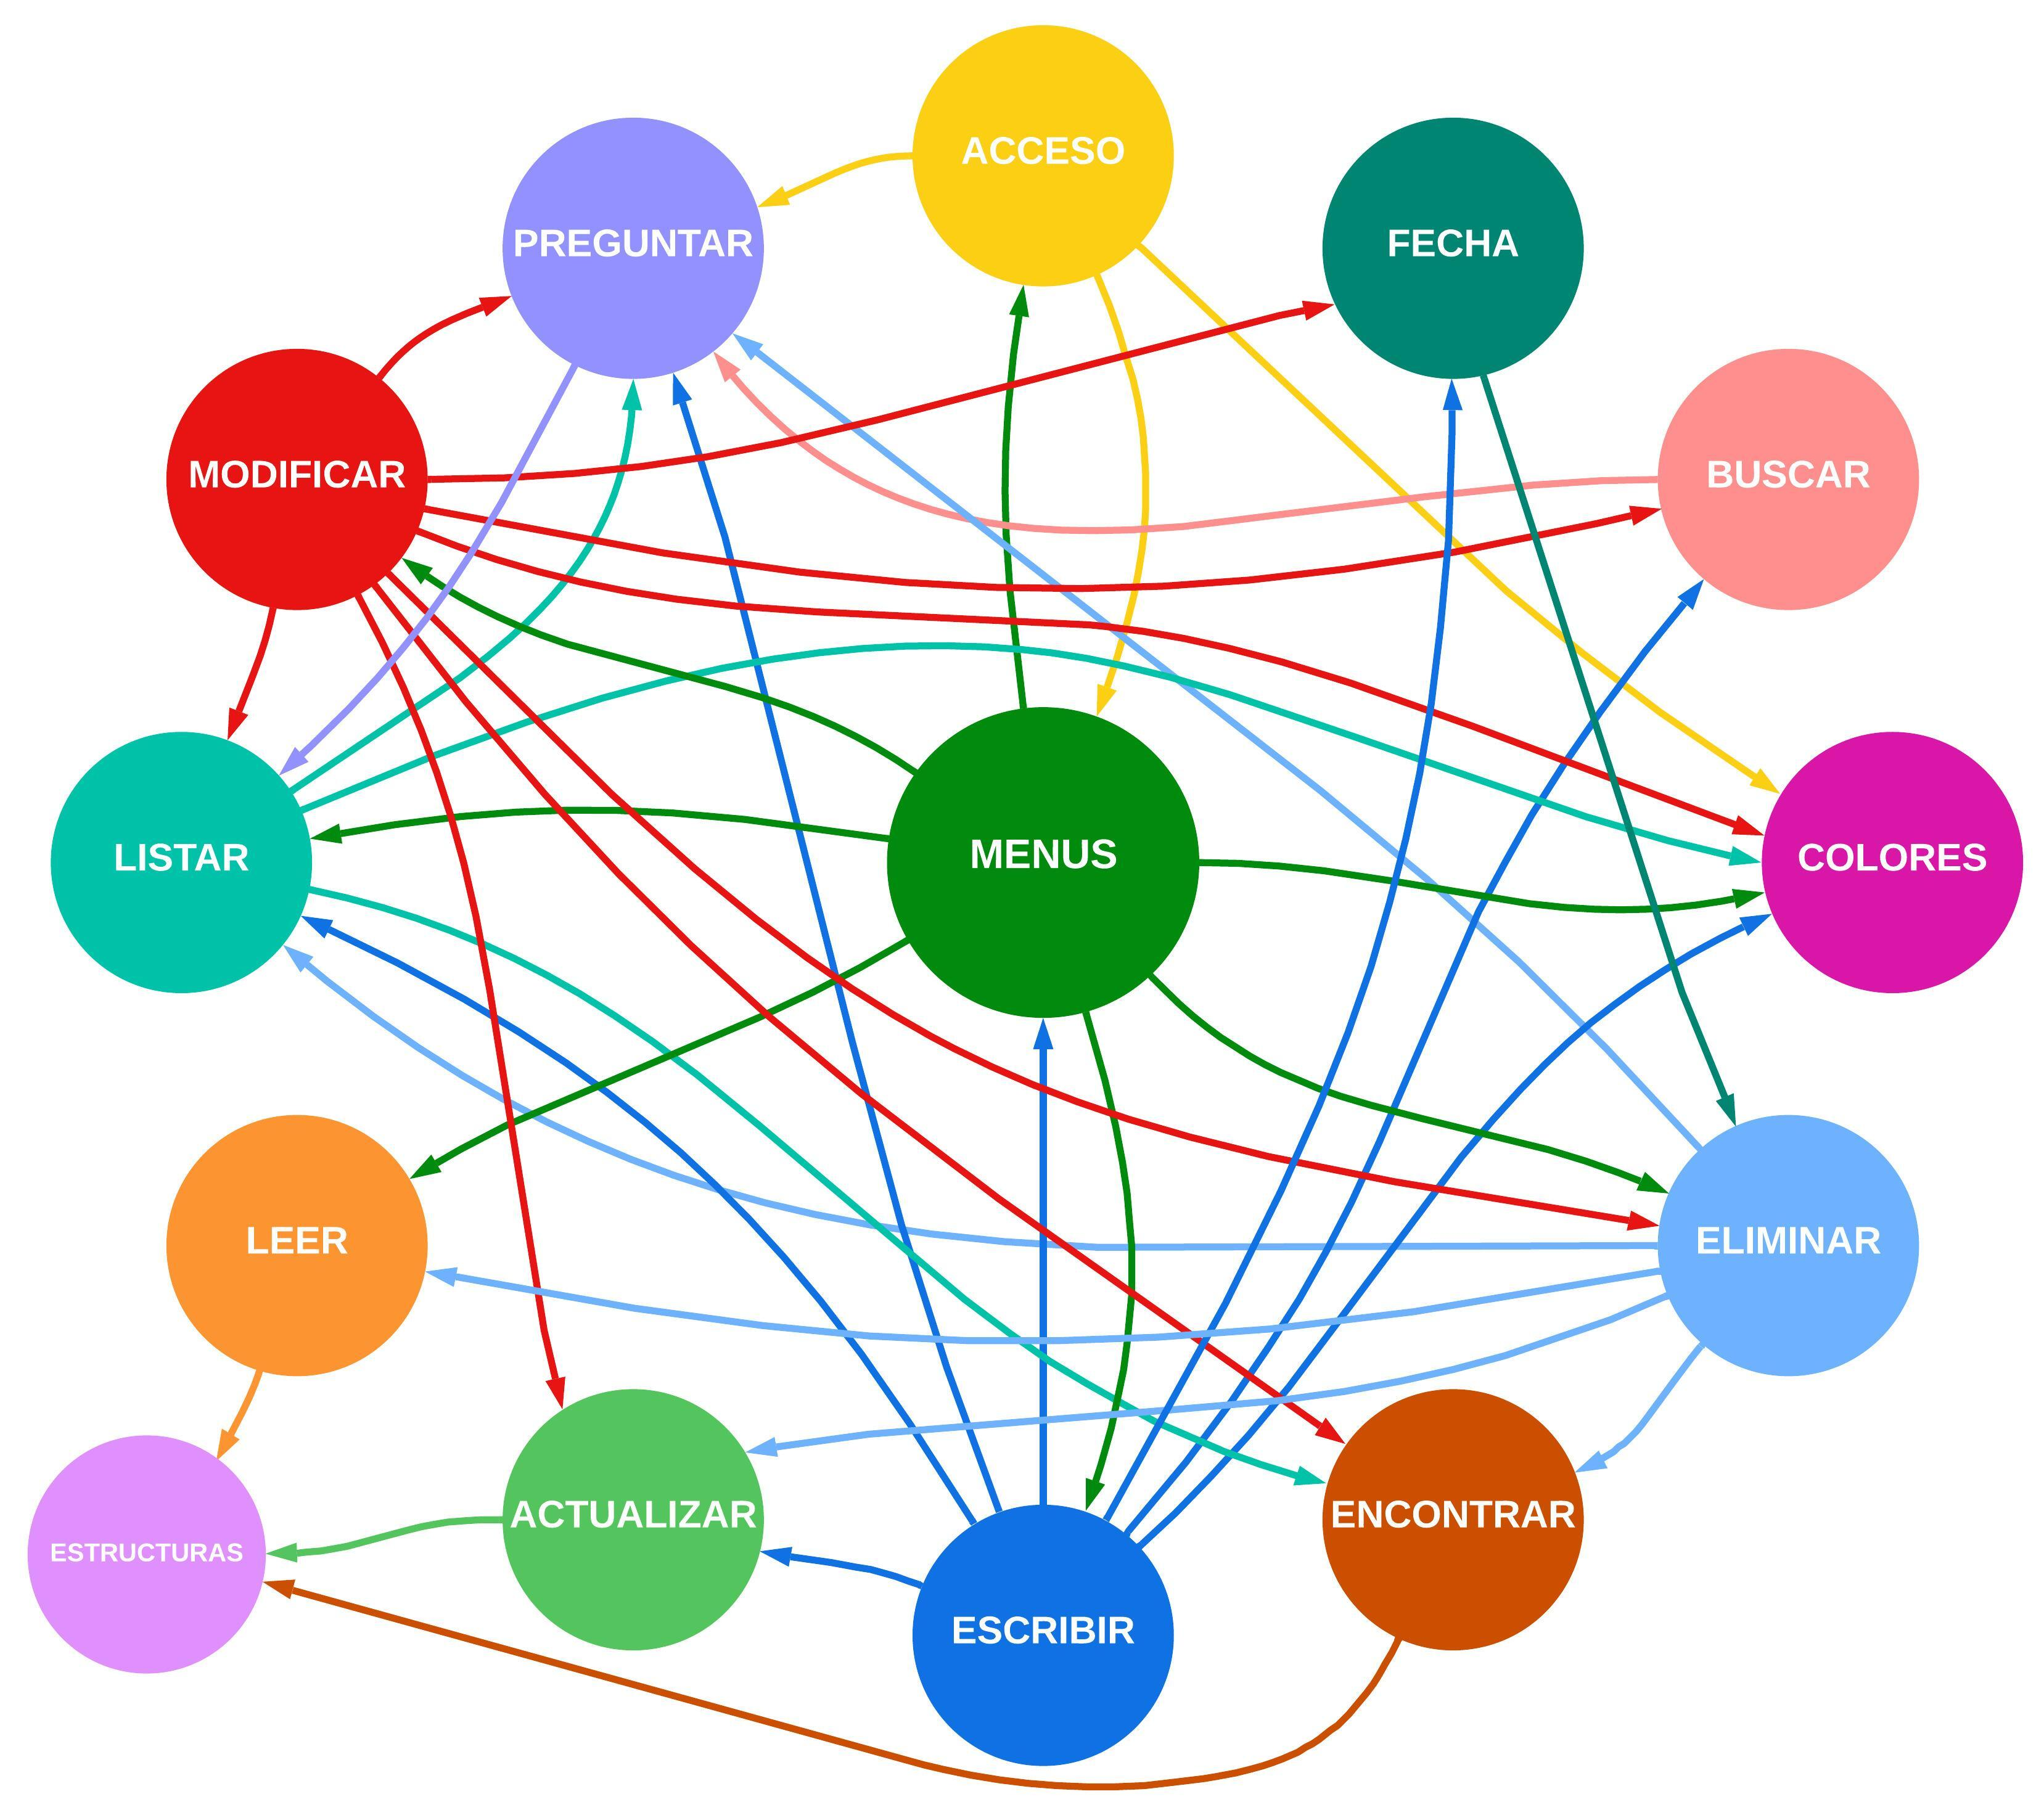
\includegraphics[width=1.1\textwidth]{FOTOS/descomposicion_modular}
\end{center}
\label{fig:DescomposicionModular}

Todos estos módulos han sido probados a fondo, introduciendo valores aleatorios, poco a poco se han ido eliminando errores, haciendo que el programa sea infalible,
y no crashee al entrar en alguna función, como pasaba anteriormente con la aplicación en fase de desarrollo.

\subsubsection{Prueba de integración}

\subsubsection{Plan de pruebas de aceptación}

En esta sección, se va a definir algunas rutas con las que usted podrá probar todos los puntos del programa. No se ha establecido una serie de datos específicos, para que así pueda probar con
todo lo que le guste, para poner a prueba el programa.

Primeramente, se encontrará el menú principal, en el que podrá acceder con las credenciales sugeridas en \ref{fig:menuPrincipal}, o puede registrar un nuevo usuario.
\begin{center}
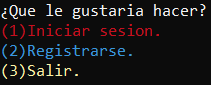
\includegraphics[]{FOTOS/menuPrincipal.png}
\end{center}
Empezaremos con el apartado de \textbf{Usuario}, introduciendo \textbf{usua1}, como usuario, y \textbf{2023}, como contraseña. 
Tras esto, se dirigirá al menú de \textbf{Pasajero}, introduciendo 1, podrá entrar en la parte de \textbf{Perfil}, en el que puede ver todos sus datos personales,
aquí puede modificar cualquier tipo de dato personal, verá que estos se actualizarán tanto en el fichero como en la estructura. Puede probar si estos se introducen correctamente, etc.
\begin{center}
    \begin{center}
      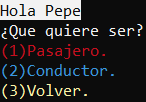
\includegraphics[]{FOTOS/menuSeleccionUsuario.png}
    \end{center}
    \begin{center}
      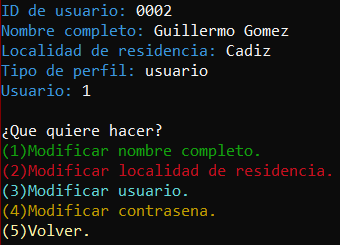
\includegraphics[]{FOTOS/menuPasajeroPerfil.png}
    \end{center}
\end{center}

Después, pulsará 2, para acceder al apartado de \textbf{Viajes}, donde podrá ver todos los viajes que tiene reservados, tras esto, puede probar las acciones del menú,
para poner a prueba el programa. Puede ver que el usuario sólo puede reservar viajes que pasan por su localidad de residencia, al igual que
no puede reservar dos veces en el mismo viaje, o que no le deja introducir una fecha anterior a la actual, etc.
\begin{center}
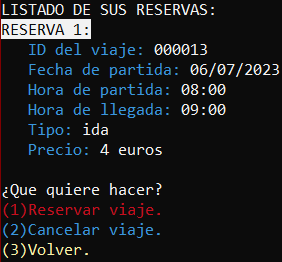
\includegraphics[]{FOTOS/menuPasajeroViaje.png}
\end{center}

Habiendo probado que todo funciona, puede volver al menú de selección de puesto, para escoger la opción de \textbf{Conductor}, introduciendo 1, entrará en el menú de \textbf{Perfil}, similar al anterior. 
\begin{center}
    \begin{center}
      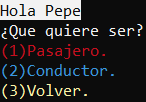
\includegraphics[]{FOTOS/menuSeleccionUsuario.png}
    \end{center}
    \begin{center}
      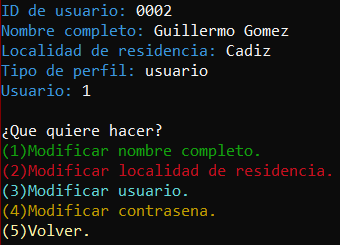
\includegraphics[]{FOTOS/menuPasajeroPerfil.png}
    \end{center}
\end{center}

Al haber probado esto, puede pulsar 2, para dirigirse al menú de \textbf{Vehículos}, donde tendrá a su vista un listado con todos los vehículos, que tiene registrados en el sistema, si lo desea,
puede explorar los menús y realizar diferentes acciones para probar el sistema, creando nuevos vehículos, o modificando y eliminando los existentes. Aquí puede ver que al eliminar un vehículo,
se eliminarán tanto sus viajes, reservas y pasos.
\begin{center}
  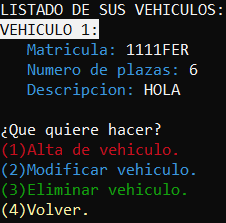
\includegraphics[]{FOTOS/menuConductorVehiculo.png}
\end{center}
Tras esto, puede dirigirse al menú de \textbf{Viajes}, introduciendo un 3, donde verá una lista de todos los viajes abiertos o iniciados que tiene en el momento, puede crear algún viaje,
para probar el sistema de creación de los mismos, o incluso modificar o anular o eliminar cualquiera. Sólo podrá anular viajes que estén abiertos, sin ninguna plaza ocupada, o finalizar,
viajes que ya estén iniciados.
\begin{center}
  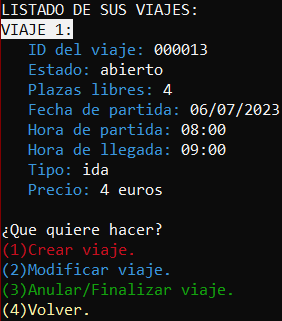
\includegraphics[]{FOTOS/menuConductorViaje.png}
\end{center}

\newpage

En segundo lugar, puede volver al menú principal, e introducir \textbf{admin}, como usuario, y \textbf{1234}, como contraseña. 
\begin{center}
    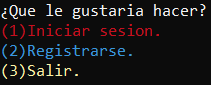
\includegraphics[]{FOTOS/menuPrincipal.png}
\end{center}

Tras esto, aparecerá un menú con 3 apartados, en \textbf{Usuarios}, podrá realizar diferentes funciones, como la creación de un usuario nuevo, o la eliminación de cualquier usuario existente,
al igual que puede modificarlos, y ver todos los usuarios del sistema, estas funciones trabajan de forma similar a las del usuario normal. 
\begin{center}
    \begin{center}
      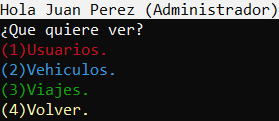
\includegraphics[]{FOTOS/menuAdmin.png}
    \end{center}
    \begin{center}
      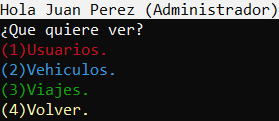
\includegraphics[]{FOTOS/menuAdmin.png}
    \end{center}
\end{center}

\newpage

Más tarde, podrá probar todo en el apartado de \textbf{Vehículos}, como la creación de nuevos vehículos al perfil de cualquier usuario, o la modificación o eliminación de vehículos existentes,
además, podrá ver una lista con todos los vehículos que hay en el sistema, o incluso ver un historial de los viajes que ha hecho un coche. 
\begin{center}
  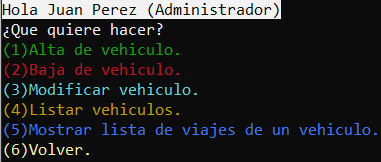
\includegraphics[]{FOTOS/menuAdminVehiculo.png}
\end{center}

Una vez haya terminado de probar todo, puede dirigirse al menú de \textbf{Viajes}, para crear un viaje con cualquier usuario del sistema, también podrá eliminar, anular o modificar
cualquier viaje que haya en la base de datos, al igual que podrá ver una lista de todos los viajes que han hecho cada usuario del sistema.
\begin{center}
  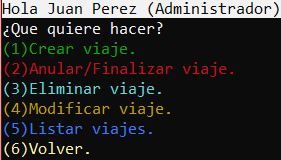
\includegraphics[]{FOTOS/menuAdminViaje.png}
\end{center}


%%%%%%%%%%%%%%%%%%%% Documentación del código %%%%%%%%%%%%%%%%%%%%


\section{Documentación del código fuente}

La documentación obtenida mediante el programa Doxygen, está aquí.


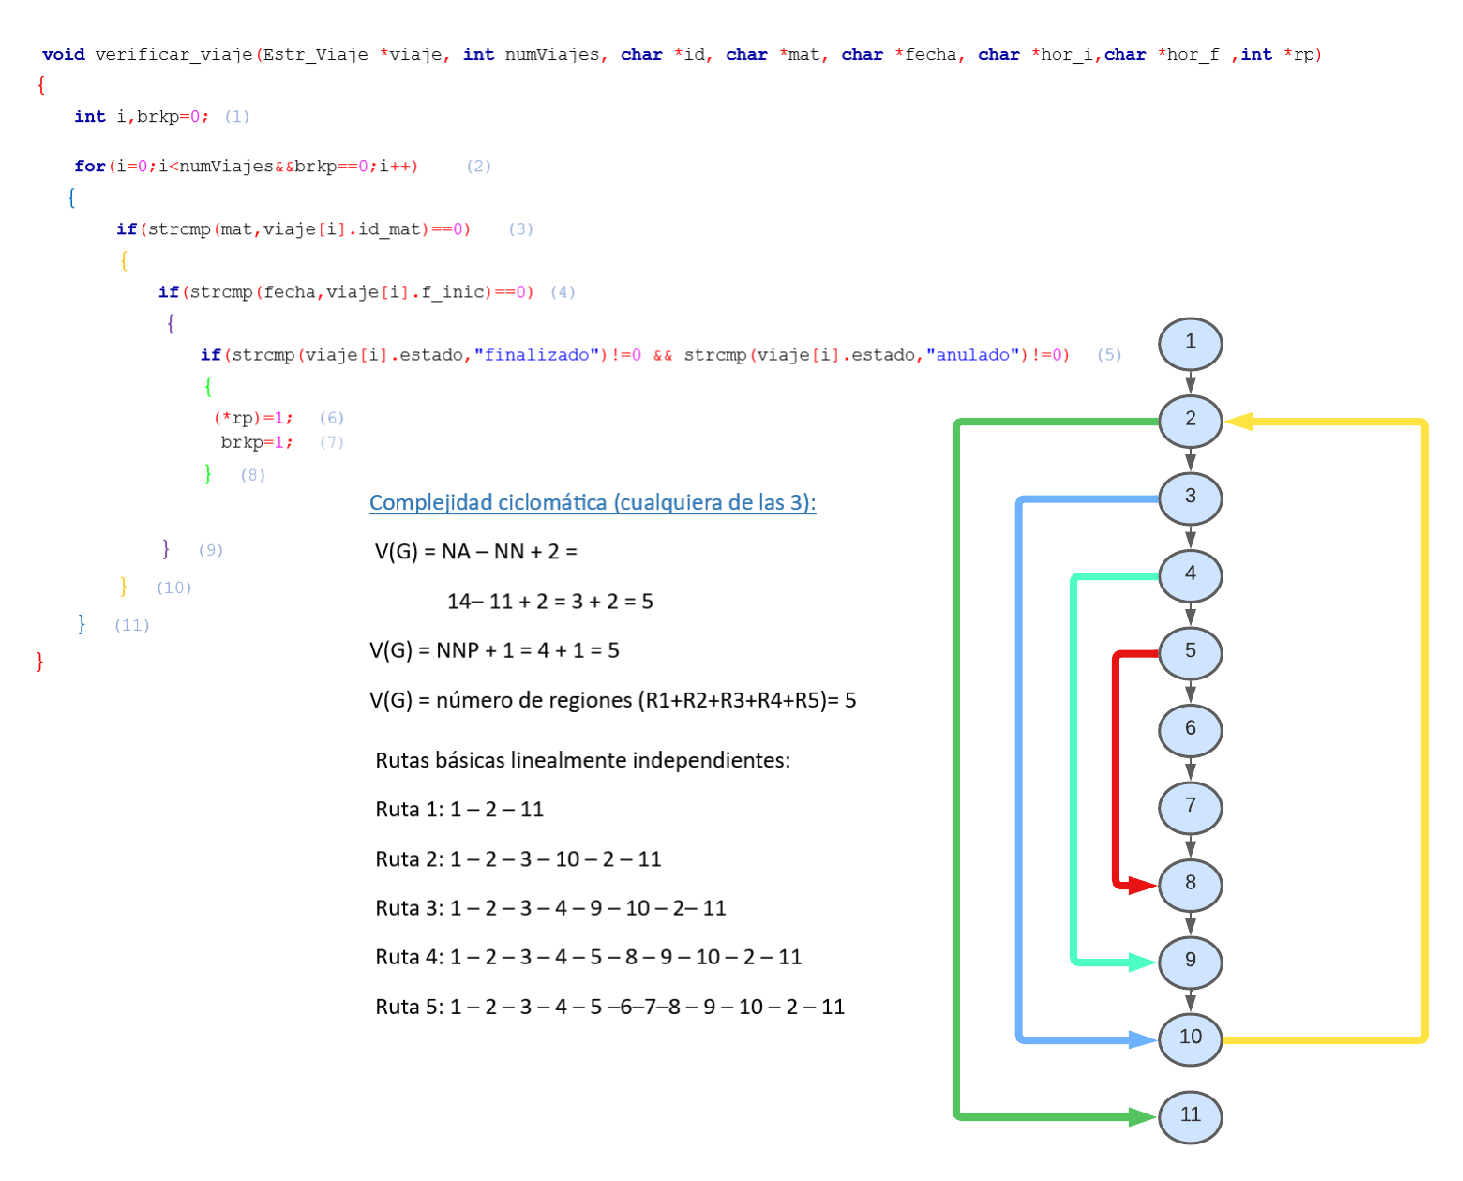
\includepdf[pages={1}]{fotos/123.pdf}

%-----------------------------------------------------------------------
% REFERENCIAS/BIBLIOGRAFÍA
%-----------------------------------------------------------------------


\nocite{*}  %Incluye todos los documentos, aunque no hayan sido citados. Lo deseable es que esté citado todo aquel documento que aparezcan en las referencias.


% Las referencias se pueden crear de dos formas. La elección de una u otra dependerá de la cantidad de citas que contenga el documento. Si va a contener muchas citas se recomienda la segunda opción.


%-----
%La primera es mediante el entorno thebibliography. Debe colocarse en la parte del documento donde deba aparecer las referencias. En este caso se ha creado un fichero donde se ha incorporado el entorno con cada entrada bibliográfica. Cada una de las entradas se crea con la instrucción bibitem. 


%\bibliographystyle{unsrtnat}

\begin{thebibliography}{}
  \bibitem[Ejemplo1, 2021]{Ejemplo1} Pérez, N. \& Ruiz, P. (2021)
  \newblock Este es un ejemplo de referencia a un artículo en revista.
  \newblock {\em Nombre de la revista en la que está publicado el trabajo}, 1(3):78-84.
  
  \bibitem[Ejemplo2, 2022]{Ejemplo2} Ruiz, P. \& Pérez, N. (2022)
  \newblock {\em Este es un ejemplo de referencia a un libro en su tercera edición (3rd ed.)}.
  \newblock Nombre de la Editorial.

  \bibitem[Ejemplo3, 2023]{Ejemplo3} Ruiz-Pérez, P.N. (2023)
  \newblock Este es un ejemplo de referencia a un artículo publicado en un congreso.
  \newblock {In \em Nombre del Congreso en el que está publicado el trabajo con todos los datos sobre su publicación, pages 1457-1563}.
  \newblock {Nombre del publicador}.

\end{thebibliography}




%-----
% La segunda es mediante BIBTEX. Está especialmente diseñada para la generación de entradas bibliográficas. Hay que crear un fichero con extensión .bib que contendrá las entradas bibliográficas. Véase el ejemplo. Hay que indicar el estilo y la ubicación del fichero. También es necesario cargar en el preámbulo el paquete para gestionar la bibliografía, en este ejemplo se ha usado natbib. 


%\bibliographystyle{apalike}
%\bibliography{Referencias.bib}



% Sea cual sea el método elegido, para incorporar una cita se utiliza el comando cite{<etiqueta>}, con la etiqueta que corresponda, como se ha visto anteriormente. 


\end{document}
